\chapter{Pré-traitement des signaux MEG}

Avant de pouvoir appliquer l'algorithme développé durant le stage, il nous faut préparer les données.
Il existe différentes librairies et logiciels qui permettent le traitement de données MEG. Il me fallait une librairie développée sous le même language de programmation que celui que j'allais utiliser pour implémenter mon algorithme, de plus je bénéficiais du travail d'un ancien stagiaire, Hiroyoshi Yamasaki, qui avait réalisé un projet de recherche sur la compréhension linguistique avec MNE-Python. J'ai donc, sous les conseils de mes encadrants, choisi d'utiliser MNE-Python (\href{https://mne.tools/stable/index.html}{https://mne.tools/stable/index.html} \cite{17} qui est une librairie complète reconnue internationalement et développée sous Python. Cette librairie permet de manipuler des données MEG avec des fonctions de pré-traitement et d'analyse déjà implémentées. J'ai travaillé sous Linux et j'ai donc créé un environnement virtuel dans lequel j'ai téléchargé les modules et librairies Python dont j'avais besoin (MNE Python, numpy) afin d'avoir un environnement de codage stable et indépendant des mises à jour système. Cela me permet également de donner précisement l'état de mon environnement avec toutes les versions des librairies et toolbox utilisées pour que mon travail puisse être reproductible, suivant ainsi les bonnes pratiques scientifiques dans ce domaine \cite{13}.
Il existe trois grandes marques de systèmes d'acquisition MEG qui ont des caractéristiques différentes. Les enregistrements issus de ces différents systèmes se présentent sous le forme de structure de données de différents formats/types. Dans notre cas, l'enregistrement des données MEG a été réalisé avec une MEG de marque CTF. Ce système d'acquisition est essentiellement caractérisé par ses capteurs dits "gradiomètres axiaux". Un des avantages de MNE-Python est qu'il permet de simplement spécifier le type de système d'acquisition pour importer les données.

\vspace{2ex}
Les données MEG sont des données très complexes qui contiennent un certain nombre de meta-données permettant au Data analyst de retrouver le protocole d'enregristrement ainsi que les paramètres d'acquisition utilisés. En effet, on crée avec MNE-Python un objet que l'on appelle raw (pour brut, les données telles qu'elles ont été enregistrées) et qui contient les données MEG relatives à l'enregistrement d'un sujet. On manipule ensuite cet objet, on peut notamment afficher les meta-données relatifs à l'enregistrement (\ref{fig3.1}) avec la commande raw.info().

\vspace{2ex}
On prendra l'exemple d'un enregistrement de la tâche visuelle pour illustrer les propos.

\begin{figure}[!ht]
    \centering
    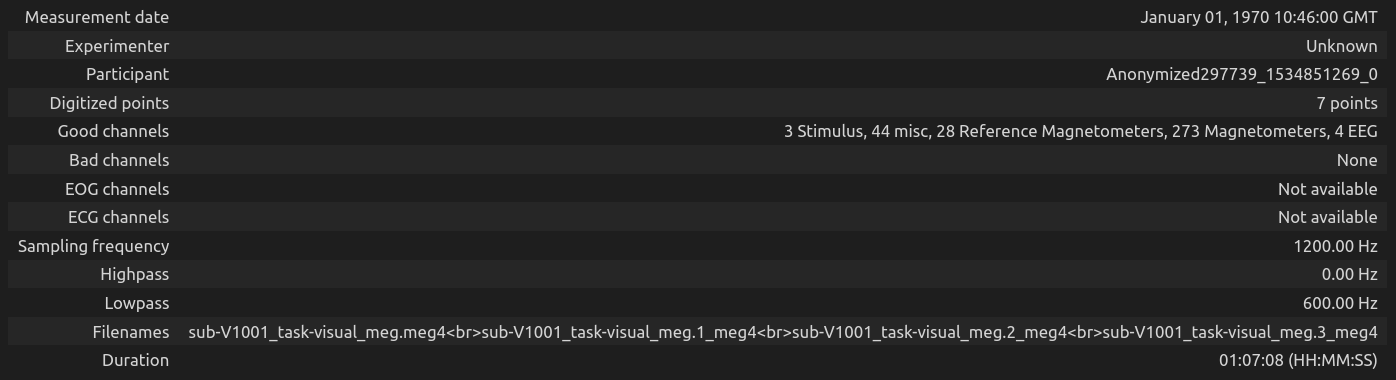
\includegraphics[width=16cm]{raw_info.png}
    \caption{Meta-données d'un enregistrement de la tâche de compréhension visuelle. On peut observer les différents canaux, y accéder aussi plus en détails, on voit aussi que la fréquence d'échantillonnage est de $1200 Hz$}
    \label{fig3.1}
\end{figure}
\section{Protocole de pré-traitement}

On présente ici (Figure \ref{fig3.2}) le protocole de pré-traitement des données qui a été mis en oeuvre durant le stage. 

\begin{figure}[!ht]
    \centering
    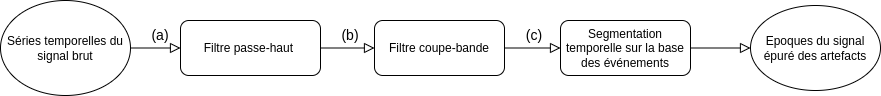
\includegraphics[width=15cm]{schema_pre_traitement.png}
    \caption{Protocole de pré-traitement des données MEG. (a) On applique d'abord un filtre passe-haut. (b) On applique un filtre coupe-bande. (c) On effectue la segmentation temporelle et donc la création d'époques des séries temporelles du signal MEG}
    \label{fig3.2}
\end{figure}

J'ai donc effectué les étapes de pré-traitement suivantes :

\begin{enumerate}
	\item Un filtre passe-haut avec une fréquence de coupure de $1 Hz$ afin de corriger la dérive lente ou "slow-drift" des séries temporelles;
	\item Un filtre coupe-bande autour de $50 Hz$ permettant de corriger le bruit des lignes éléctriques du signal MEG;
	\item Une ségmentation des séries temporelles en courtes époques en se basant sur les différentes conditions expérimentales afin d'appliquer l'algorithme mis en place durant le stage sur ces segments temporels d'intérêt.
\end{enumerate}

\section{Séries temporelles et filtre passe-haut}

Nous visualisons dans un premier temps le signal temporel pour repérer de potentiels artefacts visibles comme les battements du coeur ou les clignements des yeux.

Les artefacts limités à une plage de fréquences étroite peuvent parfois être réparés en filtrant les données. Les dérives lentes et le bruit des lignes électriques sont deux exemples d'artefacts limités à une plage de fréquences. Ce sont donc ces artefacts que nous avons traité afin de modifier le moins possible le signal d'origine et ainsi conserver de manière intacte la dynamique cérébrale.

\begin{figure}[!ht]
    \centering
    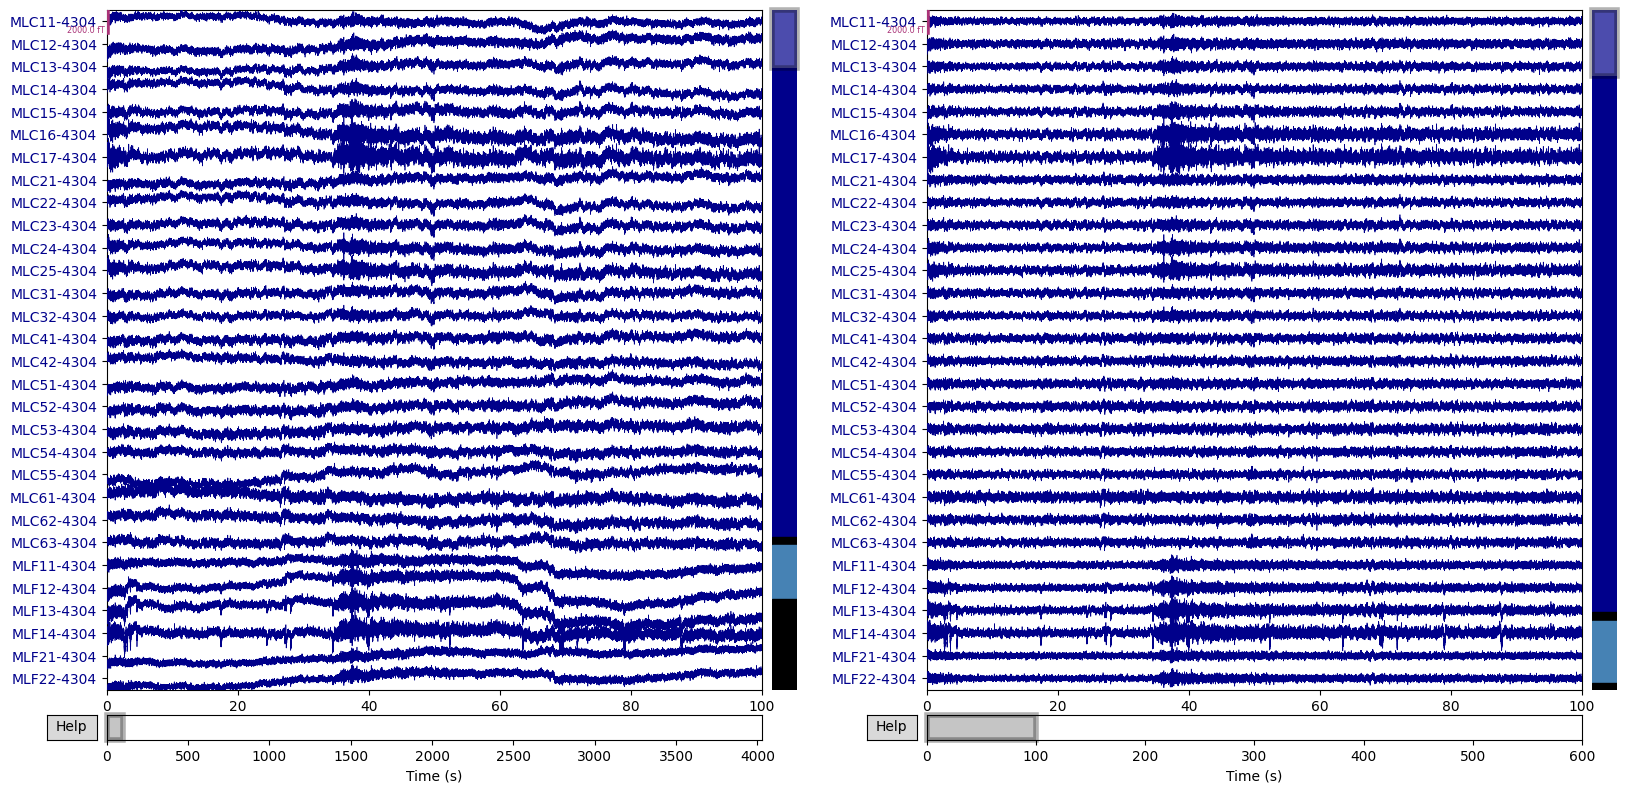
\includegraphics[width=13cm]{series_temporelles_effet_hp.png}
    \caption{A gauche, séries temporelles des différents canaux du signal MEG brut. A droite, séries temporelles après application du filtre passe-haut}
    \label{fig3.3}
\end{figure} 

On observe que les signaux ne sont pas centrés sur l'origine, ils dérivent. C'est là une dérive lente que l'on peut réparer en filtrant notre signal avec un filtre passe-haut avec une fréquence de coupure de $1 Hz$. 

\vspace{2ex}
Nous avons appliqué un filtre passe-haut pour corriger la dérive lente des séries temporelles. Par rapport, aux filtres coupe-bande, cela ne pose pas de problèmes car les activités fréquentielles du cerveau sont définies sur une plage de fréquence $\geq 1 Hz$. Après application du filtre passe-haut, le signal est à présent centré autour de 0.

\section{Spectre et filtre coupe-bande}

Il est essentiel de représenter les amplitudes en fonction des fréquences contenues dans le signal, comme en Figure \ref{fig3.4}. Ce type de représentation est appelé spectre; elle permet de mettre en évidence le contenu fréquentiel du signal.
On observe un pic à $50 Hz$ ainsi que ses harmoniques. Cette composante fréquentielle correspond au bruit dû à l'alimentation en courant du système d'acquisition, c'est le bruit des lignes électriques. Cet artefact environnemental se manifeste par des oscillations persistantes centrées autour de la fréquence de la ligne électrique, d'où le pic observé. 

\vspace{2ex}
J'ai donc utilisé un filtre coupe-bande à $50 Hz$ pour retirer la fondamentale du bruit des lignes éléctriques. J'ai fait le choix de ne pas appliquer de filtres coupe-bande pour retirer les harmoniques de cet artefact ($100 Hz, 150 Hz,...$) car même si la bande passante est très fine, cela risquerait de modifier significativement tout le signal et de perdre des informations quand à l'activité neuronale.

\begin{figure}[!ht]
    \centering
    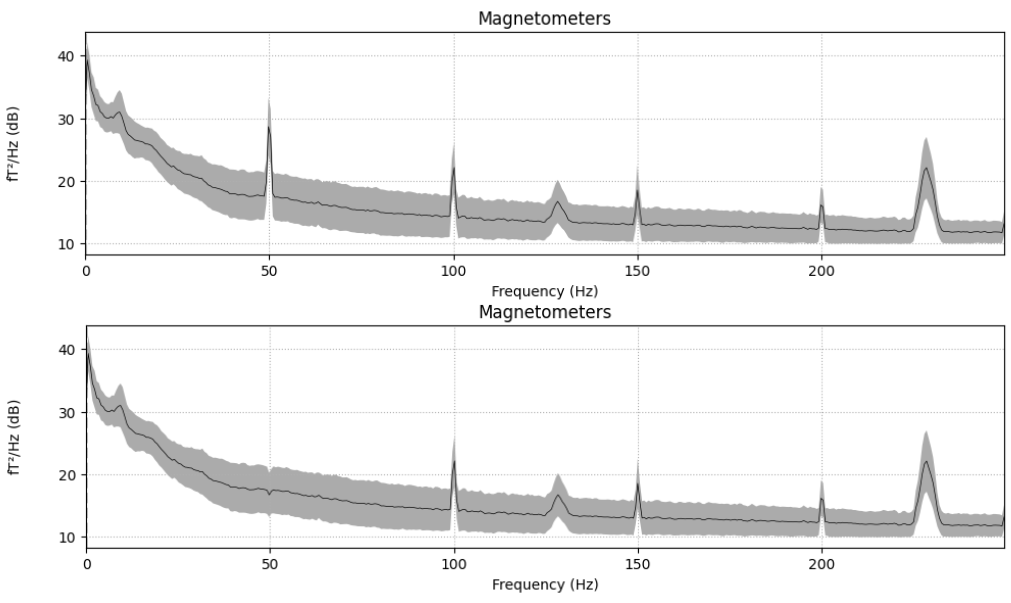
\includegraphics[width=13cm]{spectre_effet_coupe_bande.png}
    \caption{Graphe de la densité spectrale relatif à l'enregistrement d'un sujet de la tâche visuelle. En haut, le spectre du signal brut. En bas, le spectre du signal une fois le filtre coupe-bande à $50 Hz$ appliqué}
    \label{fig3.4}
\end{figure} 

\section{Segmentation temporelle du signal}

Une fois que les artefacts gênants pour l'étude ont été retirés des signaux MEG, il en va de le découper en courtes séquences que l'on appelle époques. En effet, pour réduire le rapport signal sur bruit, il faut appliquer l'algorithme développé au cours du stage sur une répétition de plusieurs segments temporels correspondants à un stimuli du même type (par exemple un mot cible d'une phrase simple), à une même condition expérimentale auquelle le sujet a été soumis. 

\vspace{2ex}
Les événements, dont on a présenté les différents types dans le chapitre précédent (Figure \ref{fig2.3}), sont une des méta-données de l'enregistrement MEG contenu dans le canal UPPT001 et nous renseigne sur la distribution des stimuli au cours du temps. Ces époques vont donc être selectionnées et découpées à partir des indexes temporels des différents événements (events). En effet, lors de l'enregistrement relatif à un sujet, il est renseigné une liste d'indexes temporels qui donne la trace du protocole expérimental. Cela permet de connaître le début d'une phrase et la caractérisation de celle-ci (simple, complexe, liste aléatoire de mots associée) et plus précisement l'apparition sur l'écran de chaque mot d'une phrase. 
Les événements sont cruciales pour l'analyse des données et un choix d'époques judicieux est indispensable pour obtenir des résultats significatifs. En effet, une fenêtre de temps trop grande, en prenant par exemple comme époque le signal MEG sur toute une phrase, a comme inconvénient de diluer l'activité cérébrale. Les premiers mots d'une phrase avant que la compréhension ne s'opère vont avoir une activité similaire à ceux d'une liste aléatoire de mots. Il est donc préférable de choisir une fenêtre de temps resserée autour de chaque mot pour définir les époques, en s'intéressant tout particulièrement aux target words.

\vspace{2ex}
On extrait les événements relatifs au protocole d'un sujet à partir du canal UPPT001 des données MEG. Cela nous permet de créer un objet event contenant les indexes temporels des différents événements. On renseigne ensuite un dictionnaire que l'on nomme event-id et dans lequel on fait correspondre les étiquettes (qui sont des entiers) des événements avec ce qu'ils signifient dans le protocole d'enregistrement (Figure \ref{fig2.3}). On peut visualiser en Figure \ref{fig3.5} le positionnement des événements dans le temps ainsi que le nombre de fois qu'ils apparaissent (sur 600 secondes d'enregistrement seulement, d'où l'absence de certains événements) :

\begin{figure}[!ht]
    \centering
    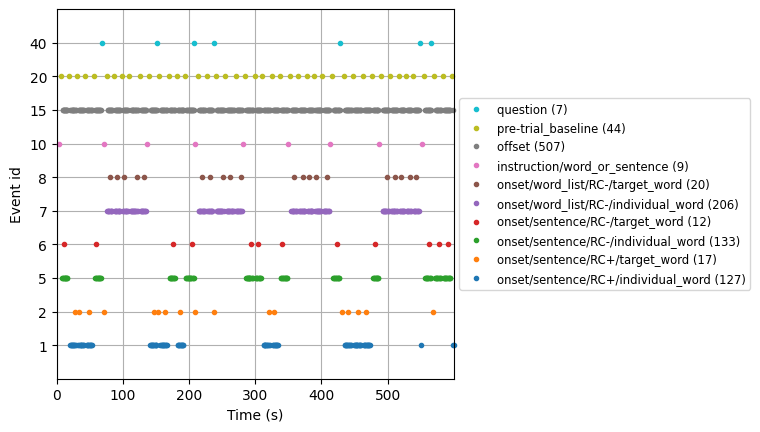
\includegraphics[width=17cm]{events_vis.png}
    \caption{Visualisation des différents événements au cours du temps d'un sujet de la tache visuelle}
    \label{fig3.5}
\end{figure} 

\vspace{2ex}
Par exemple, l'événement 5, "onset/sentence/RC+/individual-word" signifie l'affichage sur l'écran du sujet d'un mot individuel (qui n'est pas un target word) d'une phrase complexe. Sur la base de ces objets, on va créer des époques autour des événements d'intérêts.

\vspace{2ex}
Tout d'abord, on détermine l'écart maximum entre deux mots (et donc entre deux événements correspondants) d'une même phrase ou liste aléatoire de mots, cela nous permet de définir la durée que l'on choisira pour créer nos époques. Pour la tâche visuelle, on décide construire les époques en découpant le signal temporel sur chaque canaux 0.2 s avant l'affichage du mot et 1.2 s après. Ce qui nous fait des époques d'une durée de 1.4 s.

\vspace{2ex}
On discrimine ensuite les époques en fonction de l'événement d'intérêt. Dans notre cas, on construit des époques centrées autour des target words, d'autres autour des individual words, tout ça au sein des phrases simples et des listes de mots aléatoires issues de phrases simples. L'idée est de pouvoir comparer la dynamique cérébrale lors de la compréhension mot par mot entre la tâche visuelle et la tâche auditive, les phrases simples et leurs listes de mots aléatoires associées, les target words et les individual words.

\vspace{2ex}
Pour chaque époque, on a donc une matrice ayant pour lignes les 301 canaux et pour colonnes les valeurs que prennent les canaux sur le segment temporel que constitue l'époque, i.e., 1200 points.

\begin{figure}[!ht]
    \centering
    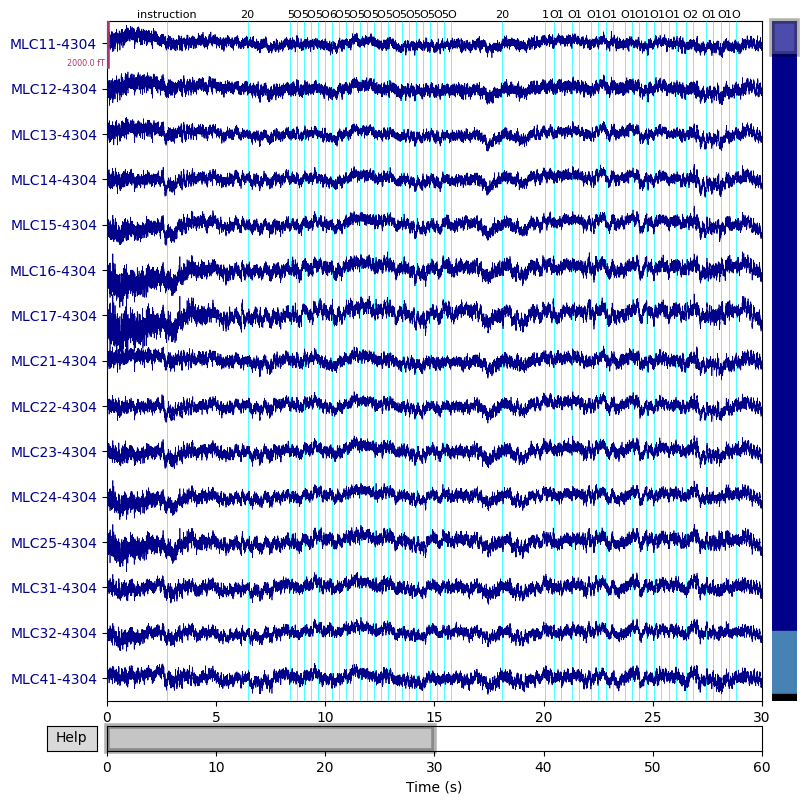
\includegraphics[width=13cm]{events_temporel.png}
    \caption{Visualisation des événements directement sur les différents canaux du signal temporel}
    \label{fig3.6}
\end{figure} 

\vspace{2ex}
Les données sont prêtes et nous avons créé les époques à partir des séries temporelles sur la base des différentes conditions expérimentales que nous souhaitons comparer. Nous pouvons à présent appliquer la partie centrale de l'algortihme mis en place durant le stage : la représentation symbolique de la dynamique cérébrale de conditions expérimentales et le calcul de l'entropie associée.
